\documentclass[a4paper,12pt,titlepage,finall]{article}

\usepackage[T1,T2A]{fontenc}     % форматы шрифтов
\usepackage[utf8x]{inputenc}     % кодировка символов, используемая в данном файле
\usepackage[russian]{babel}      % пакет русификации
\usepackage{tikz}                % для создания иллюстраций
\usepackage{pgfplots}            % для вывода графиков функций
\usepackage{geometry}		 % для настройки размера полей
\usepackage{indentfirst}         % для отступа в первом абзаце секции
\usepackage{multirow}            % для таблицы с результатами
\usepackage{amssymb}
\usepackage{minted}
\usepackage{url}
\usepackage{float}
\usepackage{graphicx}

% выбираем размер листа А4, все поля ставим по 3см
\geometry{a4paper,left=30mm,top=30mm,bottom=30mm,right=30mm}

\setcounter{secnumdepth}{0}      % отключаем нумерацию секций

\usepgfplotslibrary{fillbetween} % для изображения областей на графиках

\begin{document}
% Титульный лист
\begin{titlepage}
    \begin{center}
	{\small \sc Московский государственный университет \\имени М.~В.~Ломоносова\\
	Факультет вычислительной математики и кибернетики\\}
	\vfill
	{\Large \sc Отчет по заданию №1}\\
	~\\
	{\large \bf <<Методы сортировки>>}\\ 
	~\\
	{\large \bf Вариант double / abs asc / Shell / heap}
    \end{center}
    \begin{flushright}
	\vfill {Выполнил:\\
	студент 102 группы\\
	Соловьев~А.~И.\\
	~\\
	Преподаватели:\\
	Калинин~Г.~М.,\\
        Цыбров~Е.~Г.}
    \end{flushright}
    \begin{center}
	\vfill
	{\small Москва\\2026}
    \end{center}
\end{titlepage}

% Автоматически генерируем оглавление на отдельной странице
\begin{center}
\tableofcontents
\end{center}
\newpage

\section{Постановка задачи}

Требуется реализовать на языке C два метода сортировки массива чисел -- Shell и heap -- и провести их экспериментальное сравнение. Тип чисел в данном случае double, сортировка производится по неубыванию модулей чисел (далее под сортировкой всегда подразумевается сортировка по неубыванию модулей).\\\\
Сортировка Шелла (англ. Shell sort) -- алгоритм сортировки, являющийся усовершенствованным вариантом сортировки вставками. Идея метода Шелла состоит в сравнении элементов, стоящих не только рядом, но и на определенном расстоянии (gap) друг от друга.\\\\
Пирамидальная сортировка (англ. heap sort) -- алгоритм сортировки, суть которого состоит в превращении исходного массива в пирамиду (кучу) и последовательном перемещении наибольшего элемента этой пирамиды в конец массива.\\\\
\newpage
\section{Результаты экспериментов}
Массив 1 -- случайные отсортированные величины, массив 2 -- случайные отсортированные в обратном порядке величин, массивы 3,4 -- случайные независимые величины.
\subsection{Результаты работы Shell sort}
В Shell sort есть параметр, от которого сильно зависит количество операций -- gap sequence (последовательность расстояний). На каждом шаге берется следующее значение последовательности, обычно она убывает к 1. Ниже приведены результаты экспериментов для различных последовательностей расстояний и соответствующие им асимптотики:

\begin{table}[H]
\centering
\resizebox{\textwidth}{!}{%
\begin{tabular}{|c|c|c|c|c|c|c|c|c|}
\hline
\multirow{2}{*}{\textbf{n}} & \multirow{2}{*}{\textbf{Параметр}} & \multicolumn{4}{|c|}{\textbf{Номер сгенерированного массива}} & \multirow{2}{*}{\textbf{Среднее значение}} & \multirow{2}{*}{\textbf{Сумма средних}} \\
\cline{3-6}
& & \textbf{1} & \textbf{2} & \textbf{3} & \textbf{4} & & \\
\hline
\multirow{2}{*}{10} & Сравнения & 17 & 33 & 28 & 32 & 27.500000 & \multirow{2}{*}{49.250000} \\
\cline{2-7}
& Перемещения & 0 & 38 & 22 & 27 & 21.750000 & \\
\hline
\multirow{2}{*}{100} & Сравнения & 453 & 668 & 815 & 812 & 687.000000 & \multirow{2}{*}{1131.750000} \\
\cline{2-7}
& Перемещения & 0 & 541 & 599 & 639 & 444.750000 & \\
\hline
\multirow{2}{*}{1000} & Сравнения & 7506 & 11716 & 15139 & 14986 & 12336.750000 & \multirow{2}{*}{20602.750000} \\
\cline{2-7}
& Перемещения & 0 & 9322 & 11993 & 11749 & 8266.000000 & \\
\hline
\multirow{2}{*}{10000} & Сравнения & 115005 & 172578 & 253452 & 262963 & 200999.500000 & \multirow{2}{*}{335192.750000} \\
\cline{2-7}
& Перемещения & 0 & 127092 & 199777 & 209904 & 134193.250000 & \\
\hline
\end{tabular}%
}
\caption{последовательность расстояний \,\protect$\{\frac{n}{2^k}\}_{k=1}^{\log_2n}$}
\end{table}

Асимптотика:
$O(n^2)$ в худшем случае, и $O(n^{\frac32})$ в среднем. [1] \\

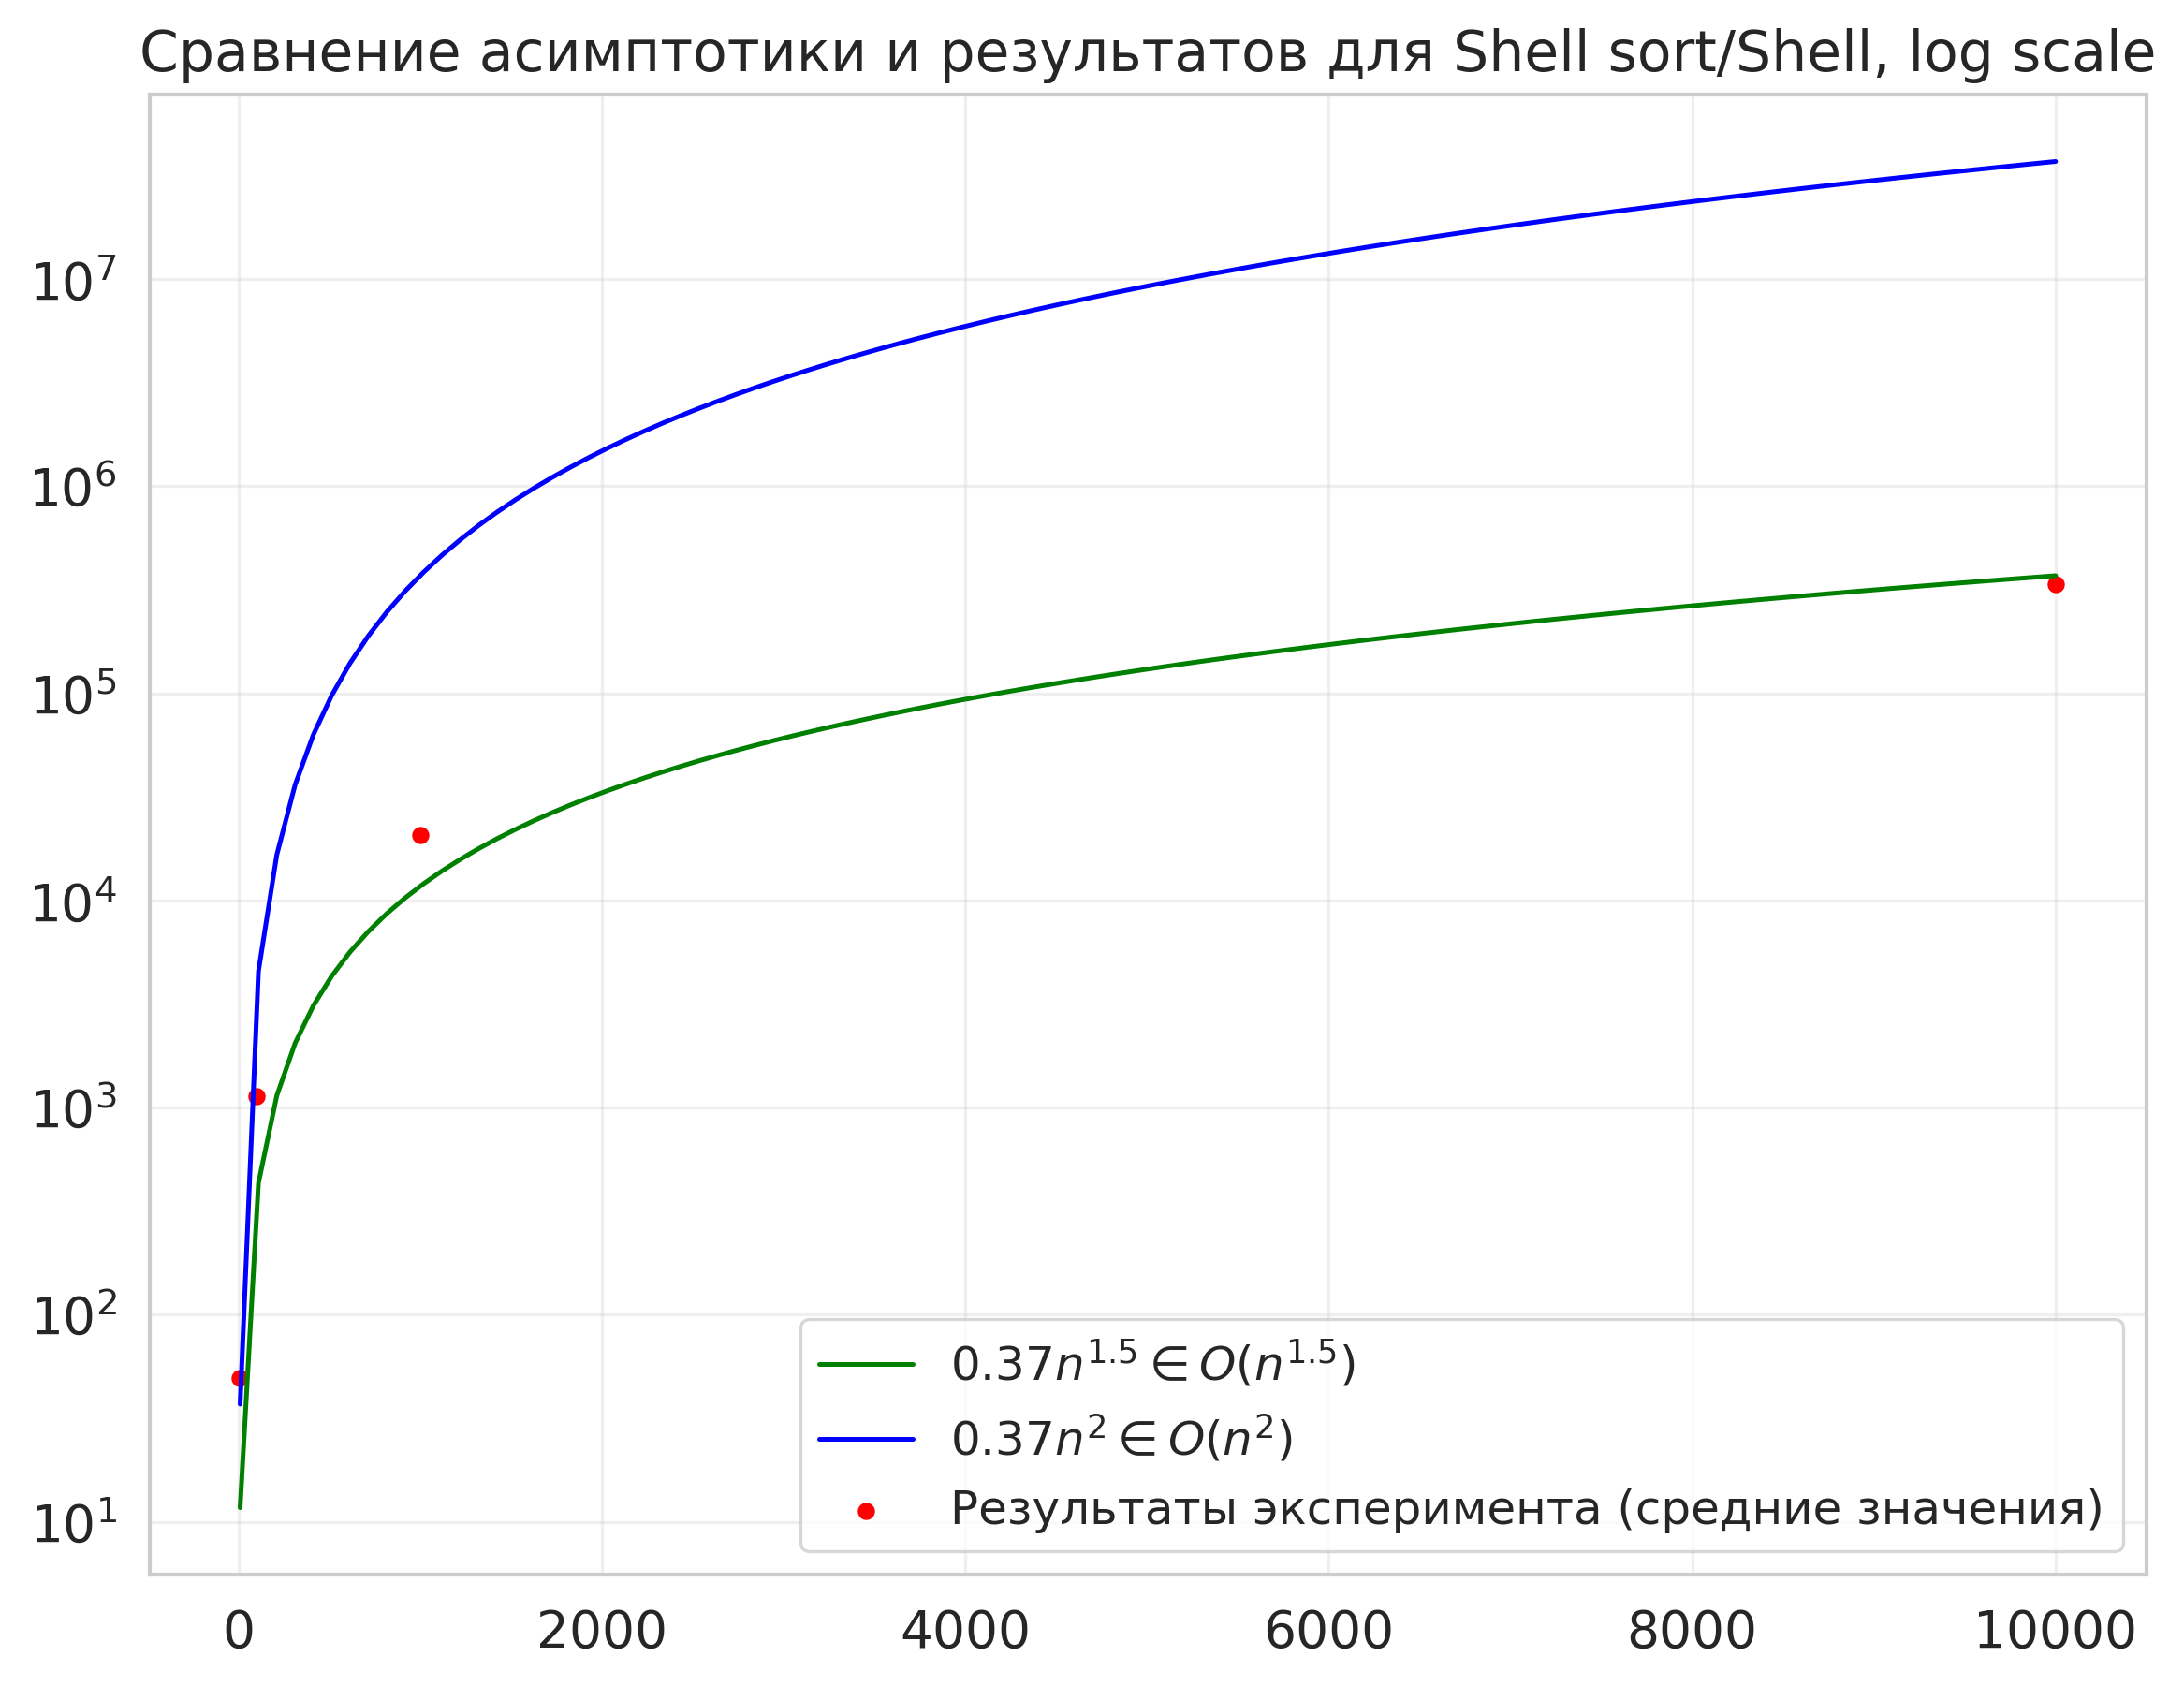
\includegraphics[width=13cm]{shell_default.png}

\begin{table}[H]
\centering
\resizebox{\textwidth}{!}{%
\begin{tabular}{|c|c|c|c|c|c|c|c|c|}
\hline
\multirow{2}{*}{\textbf{n}} & \multirow{2}{*}{\textbf{Параметр}} & \multicolumn{4}{|c|}{\textbf{Номер сгенерированного массива}} & \multirow{2}{*}{\textbf{Среднее значение}} & \multirow{2}{*}{\textbf{Сумма средних}} \\
\cline{3-6}
& & \textbf{1} & \textbf{2} & \textbf{3} & \textbf{4} & & \\
\hline
\multirow{2}{*}{10} & Сравнения & 9 & 45 & 26 & 31 & 27.750000 & \multirow{2}{*}{55.750000} \\
\cline{2-7}
& Перемещения & 0 & 54 & 27 & 31 & 28.000000 & \\
\hline
\multirow{2}{*}{100} & Сравнения & 282 & 664 & 774 & 739 & 614.750000 & \multirow{2}{*}{1130.750000} \\
\cline{2-7}
& Перемещения & 0 & 654 & 726 & 684 & 516.000000 & \\
\hline
\multirow{2}{*}{1000} & Сравнения & 4821 & 9894 & 14125 & 14712 & 10888.000000 & \multirow{2}{*}{19636.750000} \\
\cline{2-7}
& Перемещения & 0 & 8661 & 12890 & 13444 & 8748.750000 & \\
\hline
\multirow{2}{*}{10000} & Сравнения & 75084 & 121986 & 235414 & 227560 & 165011.000000 & \multirow{2}{*}{294341.500000} \\
\cline{2-7}
& Перемещения & 0 & 96520 & 214619 & 206183 & 129330.500000 & \\
\hline
\end{tabular}%
}
\caption{последовательность расстояний Кнута: \protect{$gap_{k+1} = \frac{ gap_k}{3} - 1$}}
\end{table}

Асимптотика: $O(n^{\frac{3}{2}})$. [1] \\

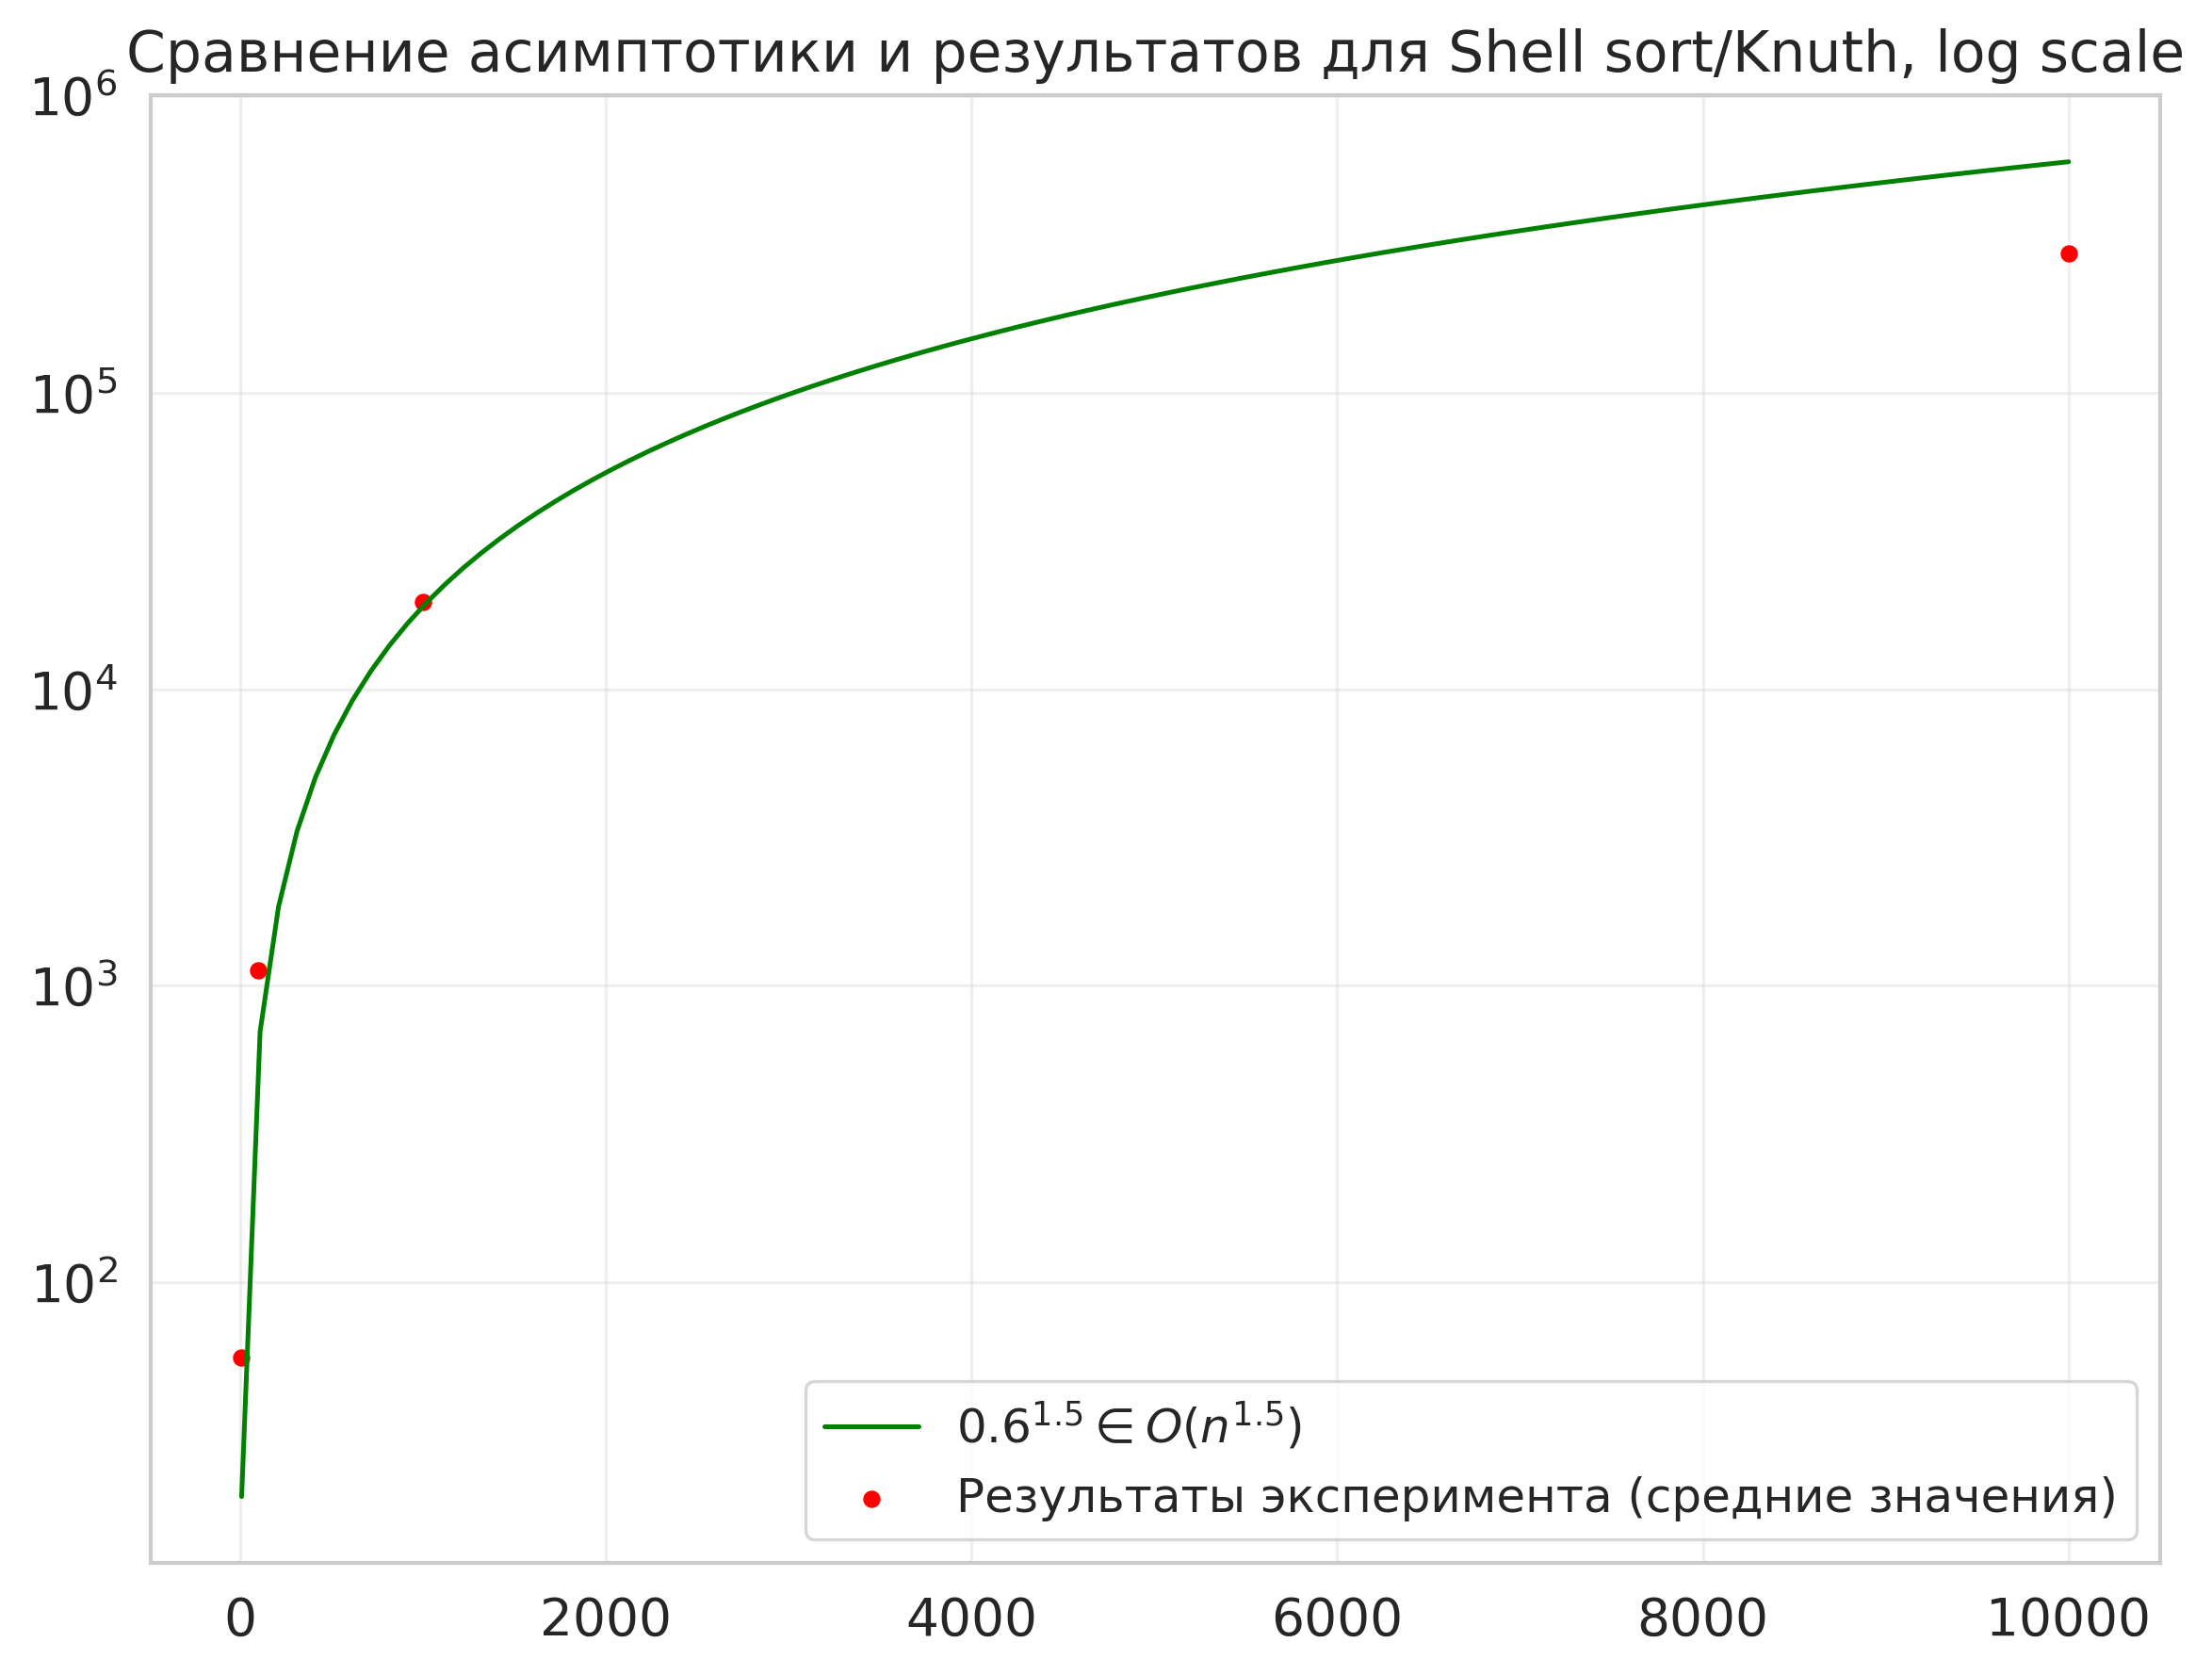
\includegraphics[width=13cm]{shell_knuth.png}
\newpage

\begin{table}[H]
\centering
\resizebox{\textwidth}{!}{%
\begin{tabular}{|c|c|c|c|c|c|c|c|c|}
\hline
\multirow{2}{*}{\textbf{n}} & \multirow{2}{*}{\textbf{Параметр}} & \multicolumn{4}{|c|}{\textbf{Номер сгенерированного массива}} & \multirow{2}{*}{\textbf{Среднее значение}} & \multirow{2}{*}{\textbf{Сумма средних}} \\
\cline{3-6}
& & \textbf{1} & \textbf{2} & \textbf{3} & \textbf{4} & & \\
\hline
\multirow{2}{*}{10} & Сравнения & 16 & 24 & 27 & 28 & 23.750000 & \multirow{2}{*}{42.000000} \\
\cline{2-7}
& Перемещения & 0 & 25 & 26 & 22 & 18.250000 & \\
\hline
\multirow{2}{*}{100} & Сравнения & 443 & 606 & 738 & 752 & 634.750000 & \multirow{2}{*}{1029.500000} \\
\cline{2-7}
& Перемещения & 0 & 433 & 552 & 594 & 394.750000 & \\
\hline
\multirow{2}{*}{1000} & Сравнения & 7498 & 10512 & 14244 & 14472 & 11681.500000 & \multirow{2}{*}{19025.000000} \\
\cline{2-7}
& Перемещения & 0 & 6997 & 11064 & 11313 & 7343.500000 & \\
\hline
\multirow{2}{*}{10000} & Сравнения & 111822 & 144764 & 247837 & 241143 & 186391.500000 & \multirow{2}{*}{304938.500000} \\
\cline{2-7}
& Перемещения & 0 & 76990 & 201691 & 195507 & 118547.000000 & \\
\hline
\end{tabular}%
}
\caption{последовательность расстояний Хиббарда -- \protect{$g_k = 2^{[log_2(n)]+1-k}-1$}}
\end{table}

Асимптотика: $\Theta(n^{\frac32})$ в худшем случае. Для среднего случая оценивается как $\Theta(n^{\frac54})$. [3], [4]

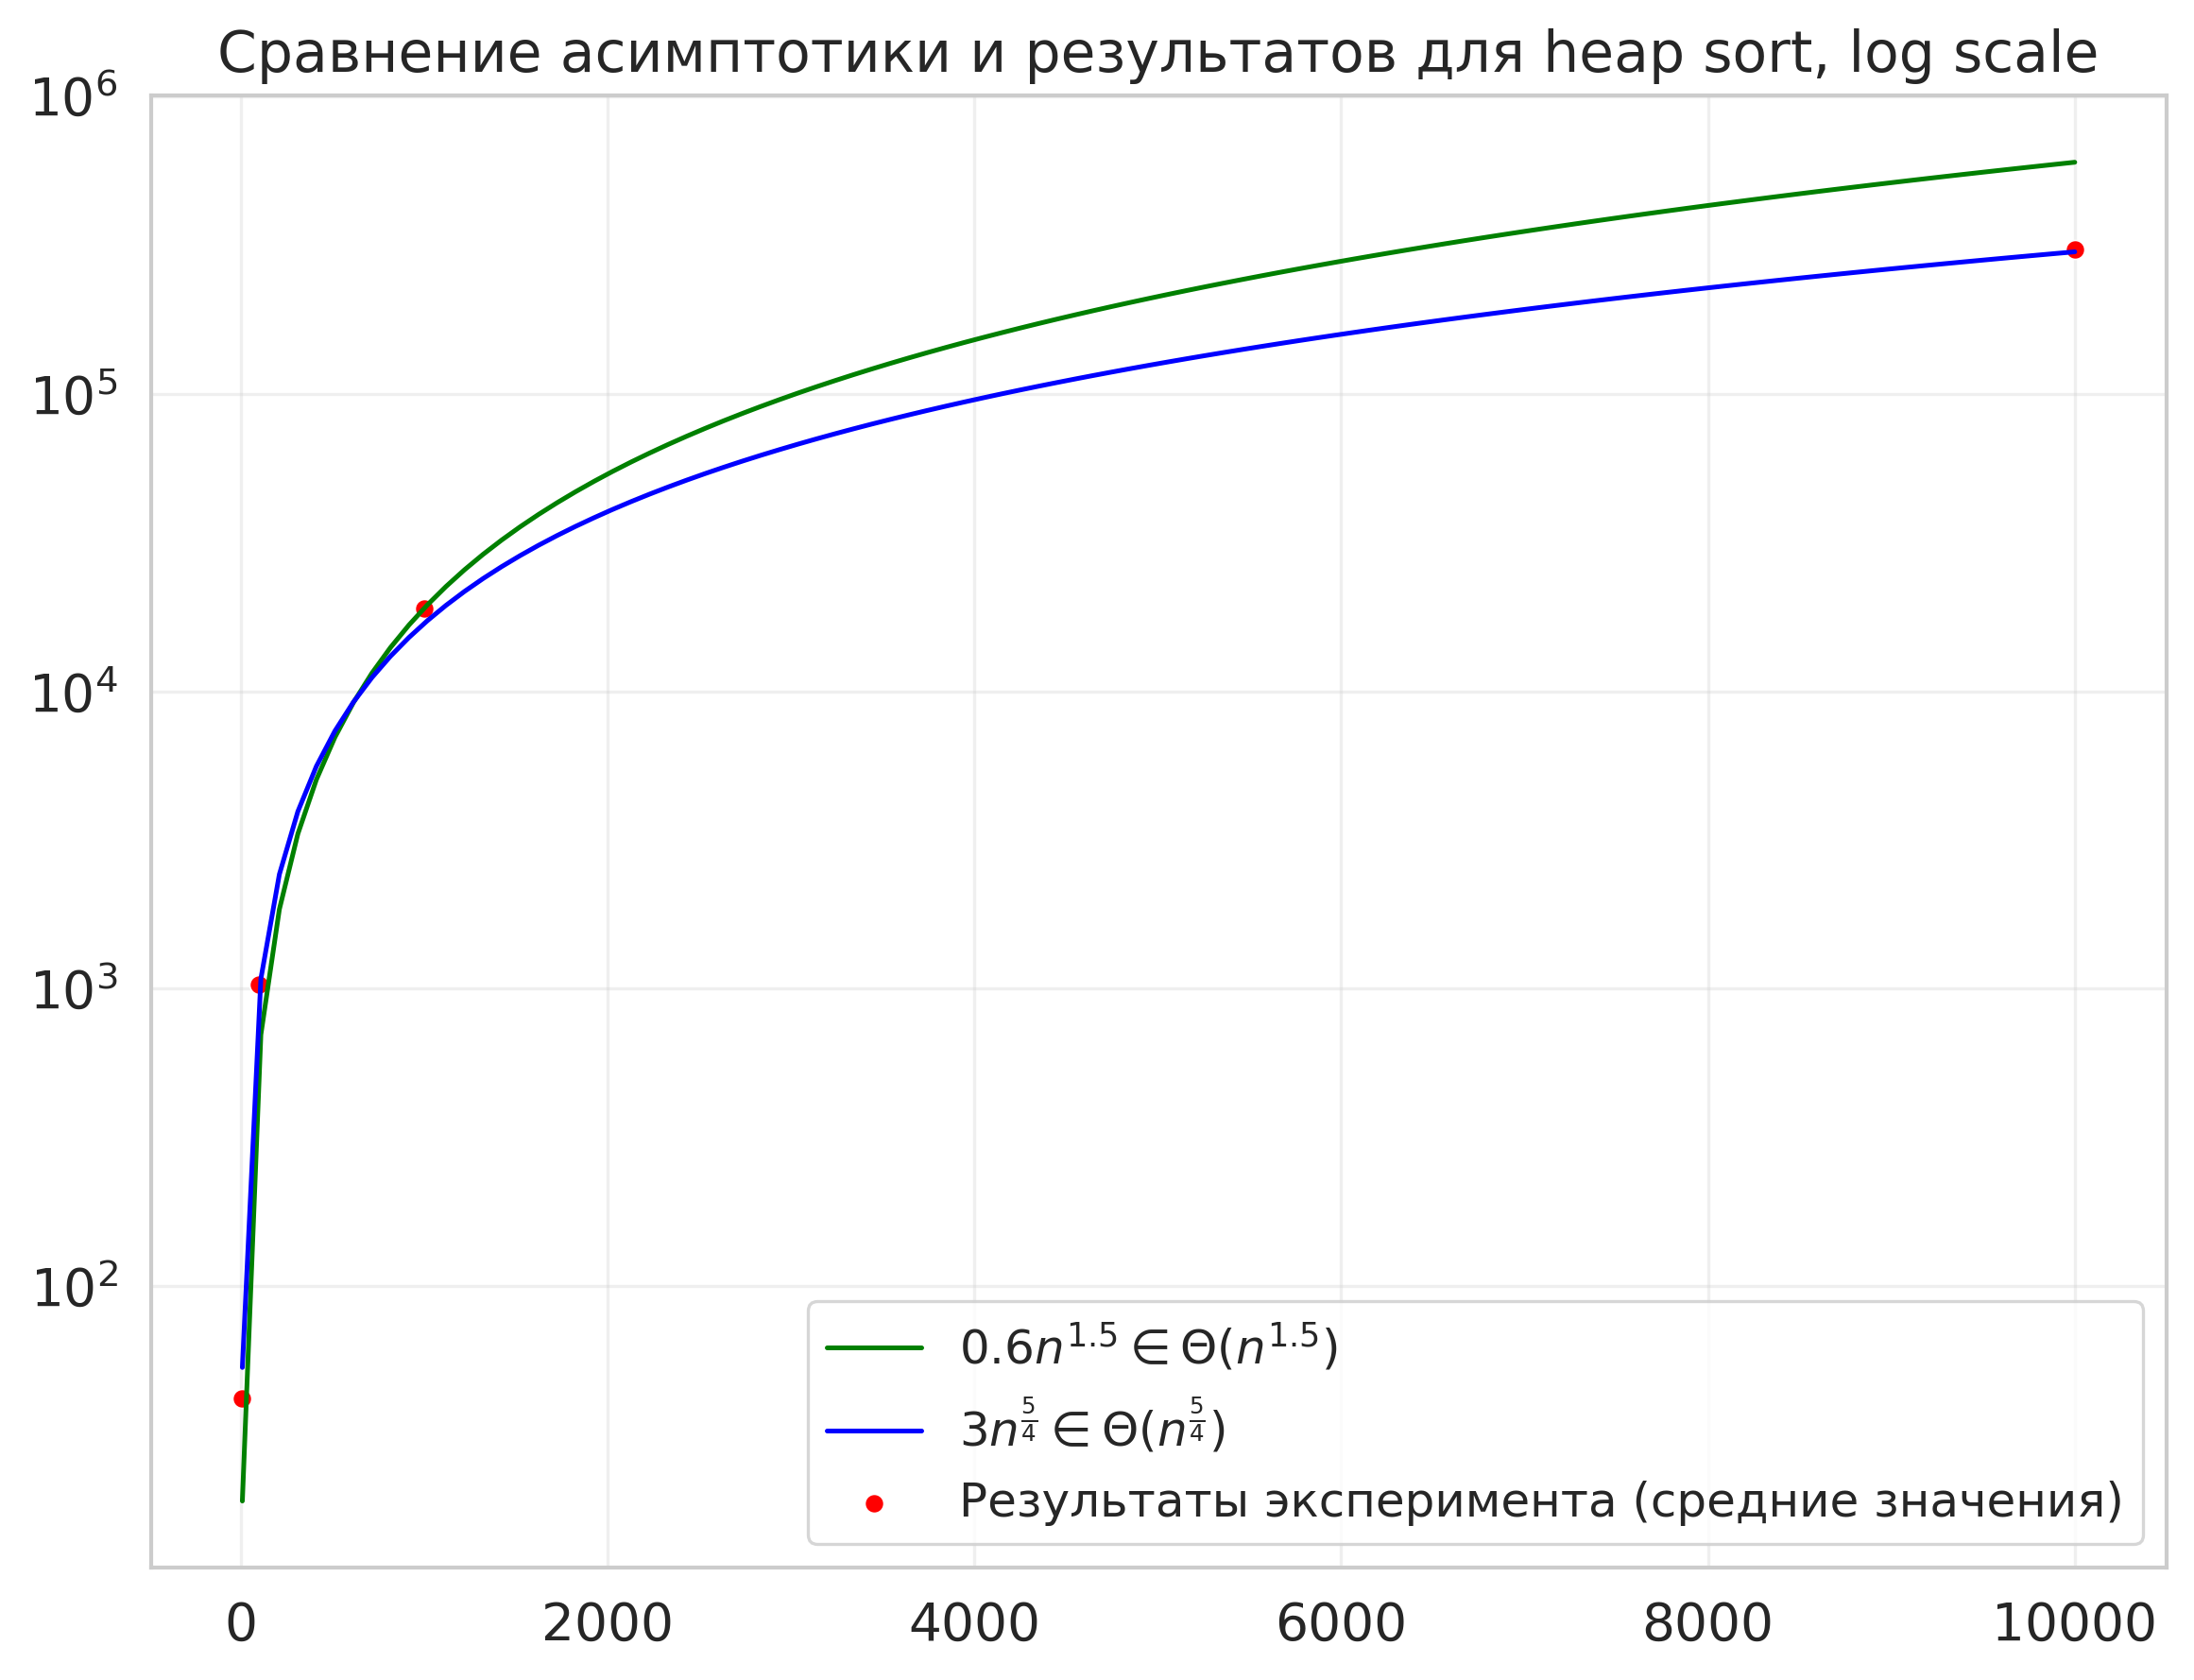
\includegraphics[width=13cm]{shell_hibbard.png}

\newpage

\begin{table}[H]
\centering
\resizebox{\textwidth}{!}{%
\begin{tabular}{|c|c|c|c|c|c|c|c|c|}
\hline
\multirow{2}{*}{\textbf{n}} & \multirow{2}{*}{\textbf{Параметр}} & \multicolumn{4}{|c|}{\textbf{Номер сгенерированного массива}} & \multirow{2}{*}{\textbf{Среднее значение}} & \multirow{2}{*}{\textbf{Сумма средних}} \\
\cline{3-6}
& & \textbf{1} & \textbf{2} & \textbf{3} & \textbf{4} & & \\
\hline
\multirow{2}{*}{10} & Сравнения & 9 & 45 & 26 & 31 & 27.750000 & \multirow{2}{*}{55.750000} \\
\cline{2-7}
& Перемещения & 0 & 54 & 27 & 31 & 28.000000 & \\
\hline
\multirow{2}{*}{100} & Сравнения & 362 & 594 & 718 & 749 & 605.750000 & \multirow{2}{*}{1039.750000} \\
\cline{2-7}
& Перемещения & 0 & 501 & 588 & 647 & 434.000000 & \\
\hline
\multirow{2}{*}{1000} & Сравнения & 6472 & 9205 & 13031 & 13130 & 10459.500000 & \multirow{2}{*}{17342.500000} \\
\cline{2-7}
& Перемещения & 0 & 6249 & 10564 & 10719 & 6883.000000 & \\
\hline
\multirow{2}{*}{10000} & Сравнения & 93083 & 129486 & 191355 & 190004 & 150982.000000 & \multirow{2}{*}{247575.750000} \\
\cline{2-7}
& Перемещения & 0 & 79546 & 154061 & 152768 & 96593.750000 & \\
\hline
\end{tabular}%
}
\caption{последовательность расстояний Ciura: \protect{$\{1, 4, 10, 23, ..., 1750, 1750 \cdot 2.25, 1750 \cdot 2.25^2, ...\}$}}
\end{table}

Асимптотика: Последовательность подобрана эмпирическим путем, поэтому для нее сложно доказать какую-либо определенную сложность. [5] \\

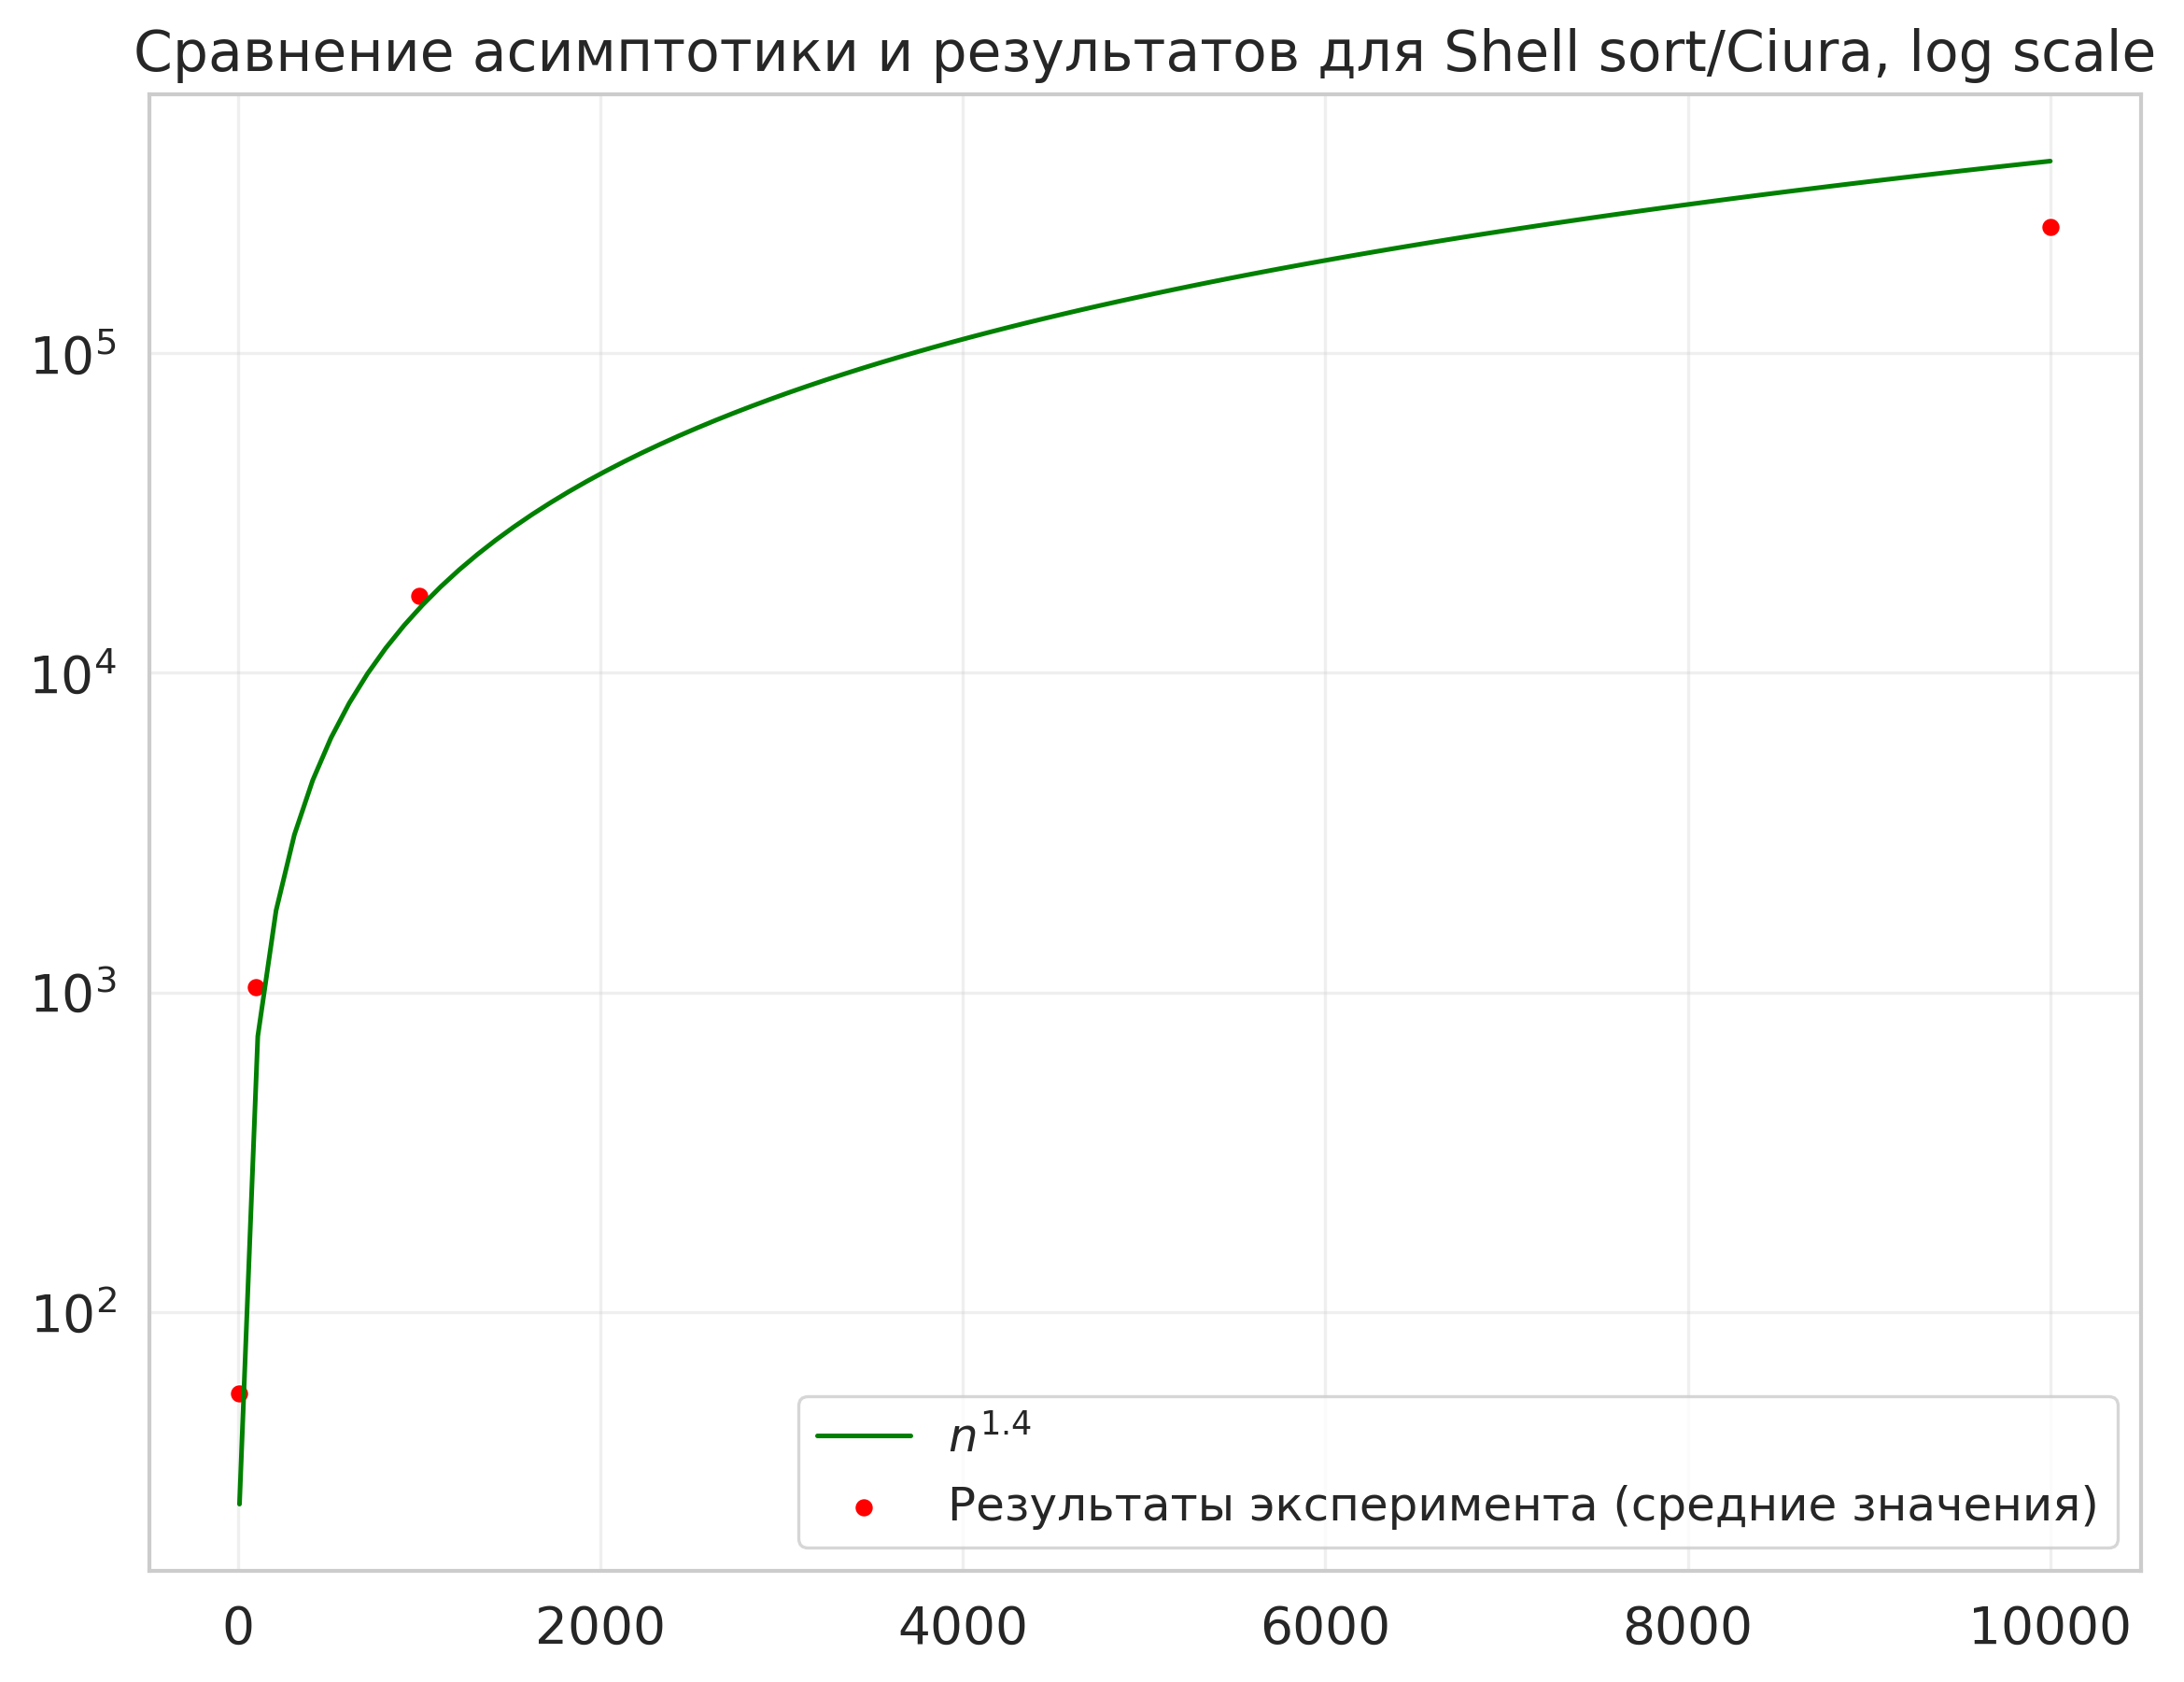
\includegraphics[width=13cm]{shell_ciura.png}

\newpage
\subsection{Результаты работы heap sort}

\begin{table}[H]
\centering
\resizebox{\textwidth}{!}{%
\begin{tabular}{|c|c|c|c|c|c|c|c|c|}
\hline
\multirow{2}{*}{\textbf{n}} & \multirow{2}{*}{\textbf{Параметр}} & \multicolumn{4}{|c|}{\textbf{Номер сгенерированного массива}} & \multirow{2}{*}{\textbf{Среднее значение}} & \multirow{2}{*}{\textbf{Сумма средних}} \\
\cline{3-6}
& & \textbf{1} & \textbf{2} & \textbf{3} & \textbf{4} & & \\
\hline
\multirow{2}{*}{10} & Сравнения & 41 & 35 & 39 & 42 & 39.250000 & \multirow{2}{*}{65.500000} \\
\cline{2-7}
& Перемещения & 30 & 21 & 28 & 26 & 26.250000 & \\
\hline
\multirow{2}{*}{100} & Сравнения & 1081 & 944 & 1033 & 1014 & 1018.000000 & \multirow{2}{*}{1598.250000} \\
\cline{2-7}
& Перемещения & 640 & 516 & 594 & 571 & 580.250000 & \\
\hline
\multirow{2}{*}{1000} & Сравнения & 17583 & 15965 & 16913 & 16910 & 16842.750000 & \multirow{2}{*}{25911.750000} \\
\cline{2-7}
& Перемещения & 9708 & 8316 & 9125 & 9127 & 9069.000000 & \\
\hline
\multirow{2}{*}{10000} & Сравнения & 244460 & 226682 & 235358 & 235182 & 235420.500000 & \multirow{2}{*}{359650.500000} \\
\cline{2-7}
& Перемещения & 131956 & 116696 & 124201 & 124067 & 124230.000000 & \\
\hline
\end{tabular}%
}
\caption{Результаты работы Heap sort}
\end{table}

Асимптотика: В худшем, среднем и лучшем случаях -- $n\;log\,n$.\\
Доказательство:
Операция <<окучивания>> требует $O(log\,n)$, применяя ее для каждого элемента, получаем $O(n\;log\,n)$; повторяем два раза: при создании кучи и при самой сортировке, получаем в сумме $O(2\cdot n\;log\,n)=O(n\;log\,n)$.$\blacksquare$

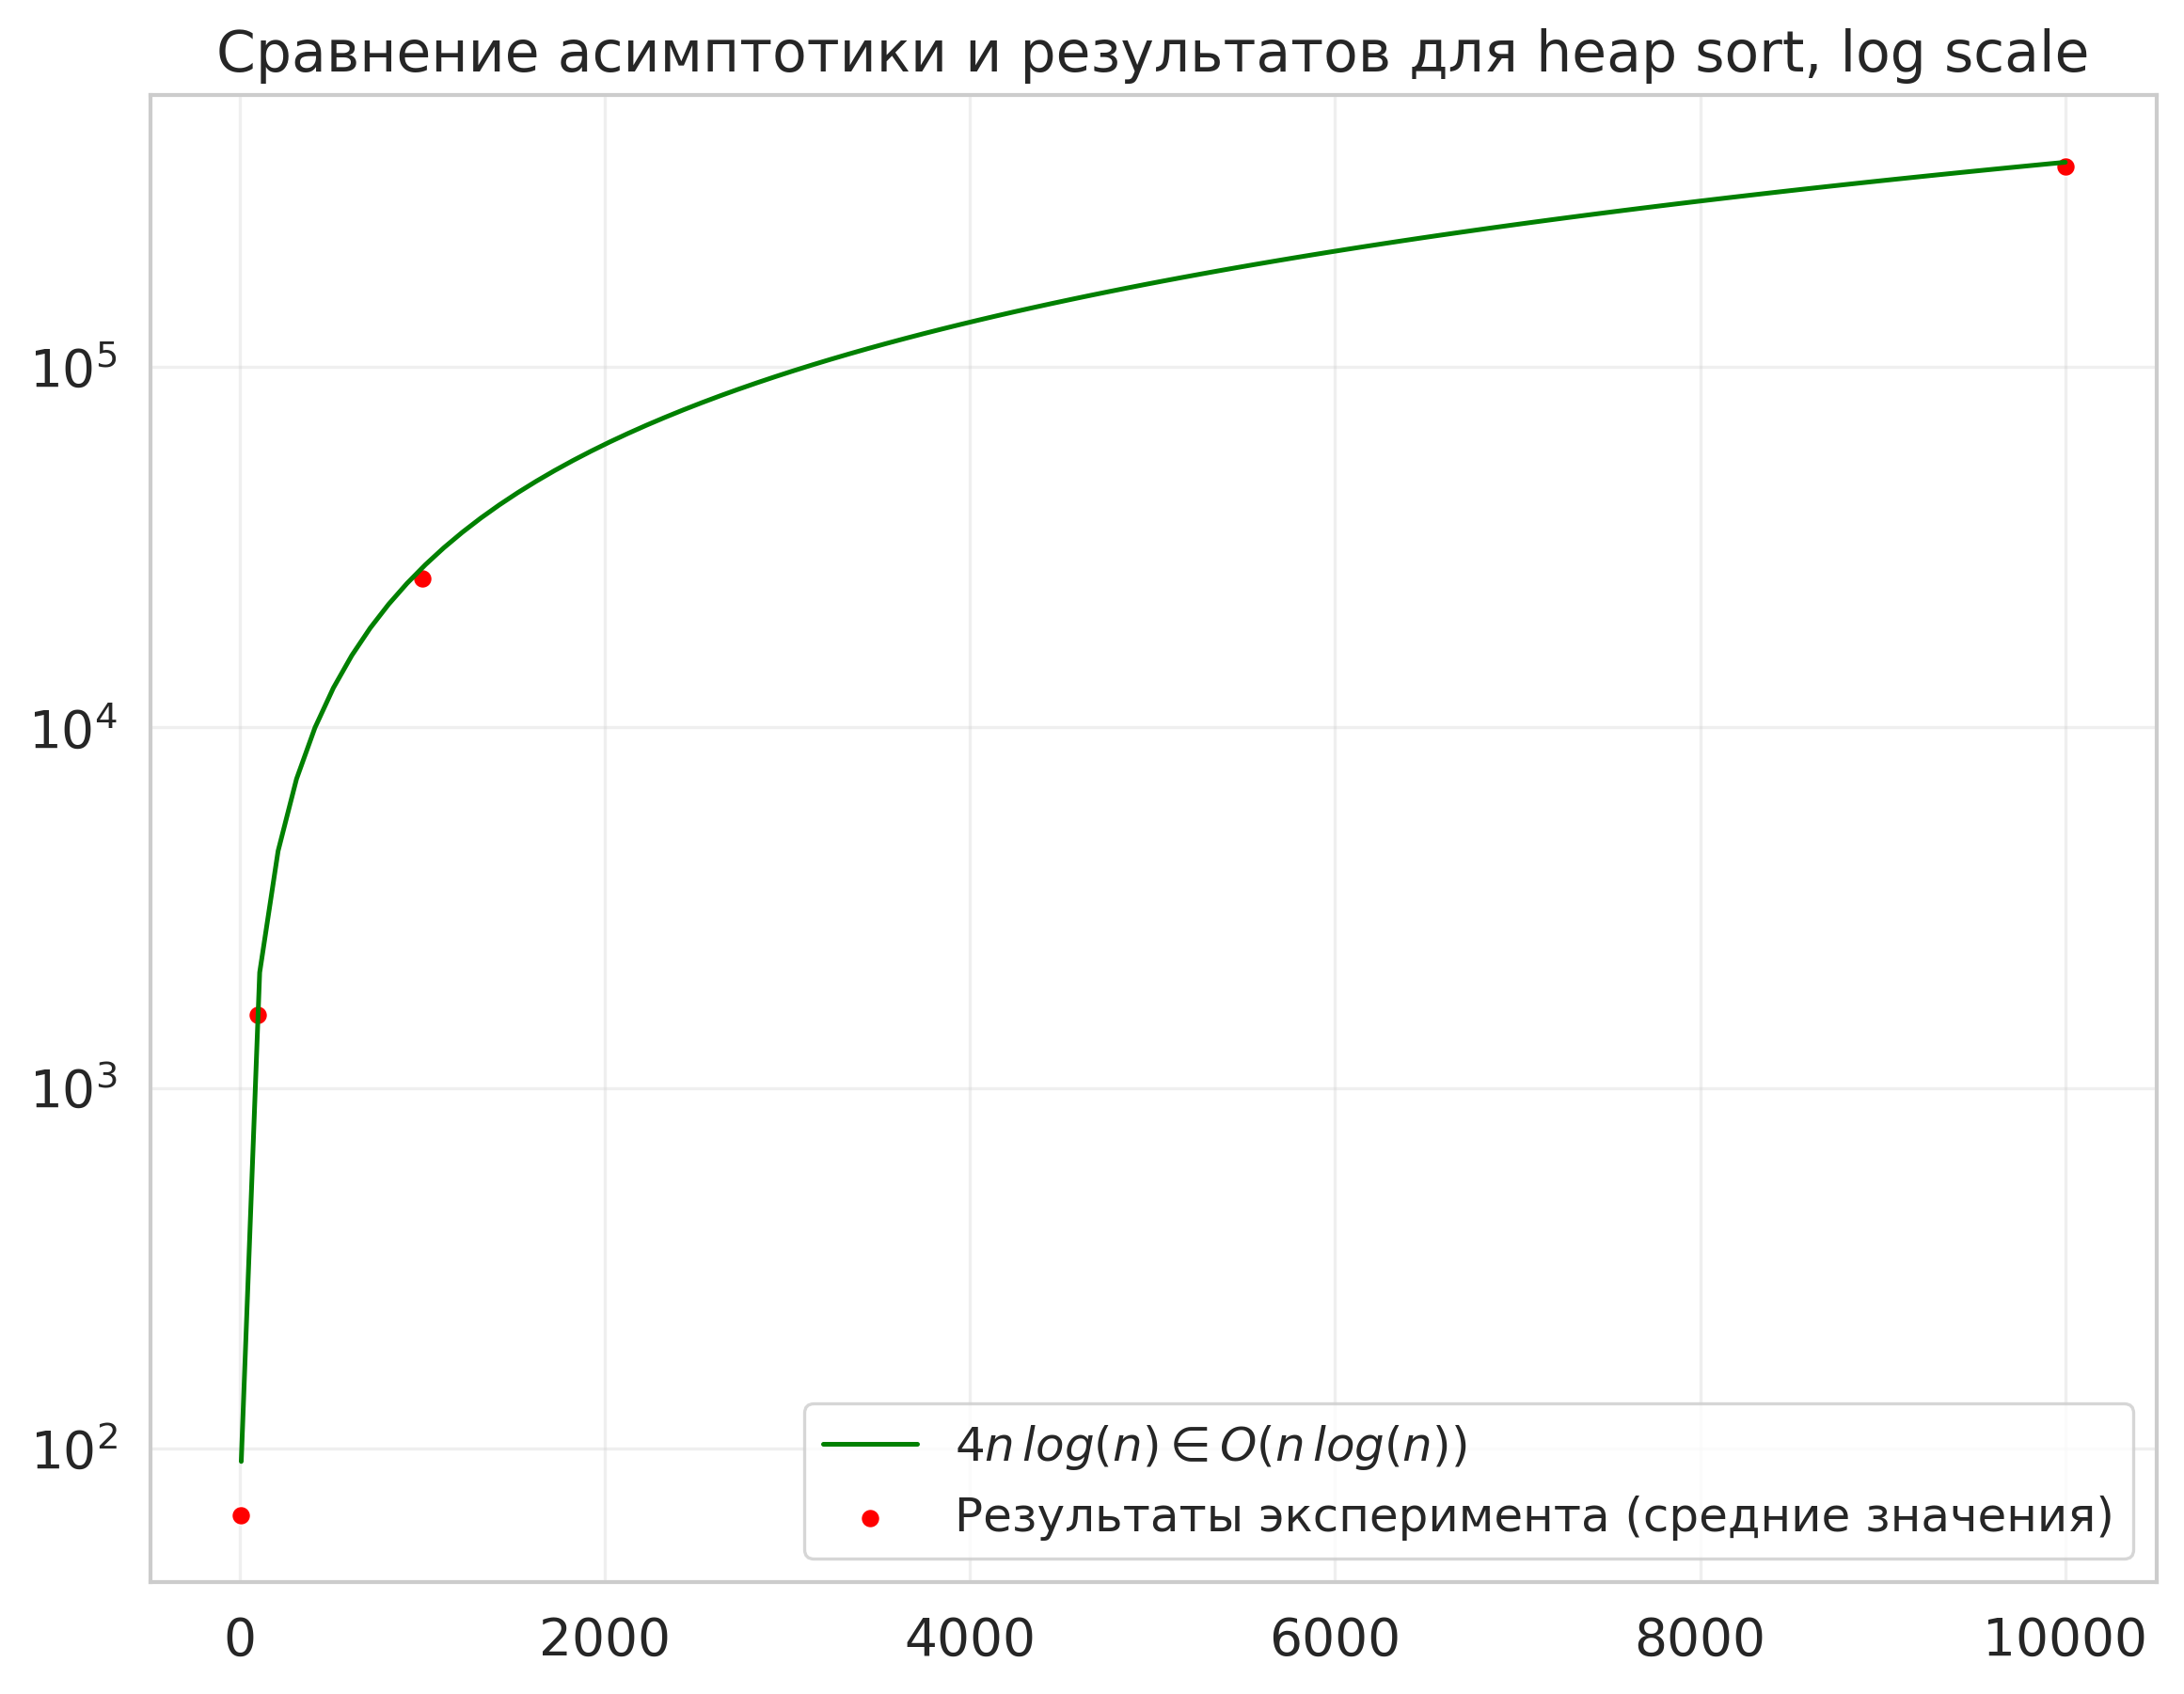
\includegraphics[width=13cm]{heap.png}

\subsection{Выводы}
По среднему значению выигрывает Shell sort с Ciura gap sequence. \\
Heap sort явно хуже Shell на небольших массивах; с увеличением количества элементов heap делает меньше перемещений, но больше сравнений, поэтому они примерно равны по числу операций. \\
\clearpage
\newpage

\section{Структура программы и спецификация функций}
Для ознакомления со структурой программы см. документацию [6].
\newpage

\section{Отладка программы, тестирование функций}
Для каждой длины $n \in \{10, 100, 1000, 10000\}$ были составлены массивы: отсортированный (лучший случай), отсортированный в обратном порядке (худший случай), и 2 случайных массива. Тестирование всех сортировок производилось на одних массивах для объективной оценки. Проверялась отсортированность и полнота (сохранение элементов) массива.
\newpage

\section{Анализ допущенных ошибок}
Проверка программы на утечки памяти:
\begin{minted}[frame=single, linenos, breaklines=true, fontsize=\small]{bash}
==190092== 
==190092== HEAP SUMMARY:
==190092==     in use at exit: 0 bytes in 0 blocks
==190092==   total heap usage: 197 allocs, 197 frees, 2,178,104 bytes allocated
==190092== 
==190092== All heap blocks were freed -- no leaks are possible
==190092== 
==190092== For lists of detected and suppressed errors, rerun with: -s
==190092== ERROR SUMMARY: 0 errors from 0 contexts (suppressed: 0 from 0)
\end{minted}
(утечек нет).\\\\
Ошибки:
в предыдущей версии программы была допущена ошибка в формировании Ciura sequence:
\begin{minted}[frame=single, linenos, breaklines=true, fontsize=\small]{bash}
int
gap_ciura(int k, int len) {
    int seq[] = {1, 4, 10, 23, 57, 132, 301, 701, 1750}; // 9 elements
    return seq[10 - k];
}
\end{minted}
При $k=1$ программа уходила за границу массива в стек, находила там значение и использовала его как gap. Что интересно, при этом Ciura gap получала меньше операций на тесте при $n=10000$ -- 152000 сравнений и 104000 перемещений, против 163000 сравнений и 120000 перемещений в новой версии без бага:
\begin{minted}[frame=single, linenos, breaklines=true, fontsize=\small]{bash}
int
gap_ciura(int k, int len) {
    int seq[] = {1, 4, 10, 23, 57, 132, 301, 701, 1750};
    int i = 8;
    while (i > 0 && len <= seq[i]) {
        --i;
    }
    return seq[i - k + 1]; // k >= 1
}
\end{minted}
Решилось добавлением новых gap'ов: $\{1, 4, 10, 23, 57, 132, 301, 701, 1750, 3938, 8860\}$ (можно продолжать и далее - новые элементы после $1750$ получаются как $1750\cdot 2.25^m$).

\newpage
\begin{raggedright}
\addcontentsline{toc}{section}{Список цитируемой литературы}
\begin{thebibliography}{99}
\bibitem{cs} Knuth, D. E. The Art of Computer Programming.
    Vol. 3: Sorting and Searching.~---Addison-Wesley (1998), 84--91.
\bibitem{cs} Shell, D. L.: A high-speed sorting procedure. Communications of the ACM 2
(1959), 30–32.\\
    URL: \url{https://web.archive.org/web/20170830020037/http://penguin.ewu.edu/cscd300/Topic/AdvSorting/p30-shell.pdf}
\bibitem{cs} Pratt, V. R.: Shellsort and Sorting Networks (1972) \\
    URL: \url{https://apps.dtic.mil/sti/tr/pdf/AD0740110.pdf}
\bibitem{cs} Папернов А.А., Стасевич Г.В.: Об одном методе упорядочивания информации в запоминающих устройствах цифровых машин \\
    URL: \url{https://www.mathnet.ru/links/70f3017dee65e76e20d95c70ee67cc79/ppi751.pdf}
\bibitem{cs} Ciura, M.: Best Increments for the Average Case
    of Shellsort (2001) \\
    URL: \url{https://web.archive.org/web/20180923235211/http://sun.aei.polsl.pl/~mciura/publikacje/shellsort.pdf} \\
\bibitem{cs}
        \url{https://artteam8.github.io/Shell-vs-heap}
\end{thebibliography}
\end{raggedright}

\end{document}
